%%%%%%%%%%%%%%%%%%%%%%%%%%%%%%%%%%%%%%%%%%%%%%%%%%%%%%%%%%%%%%%%%%%%%%%%%%%%%%%%
\chapter{Orbital Mechanics}
%%%%%%%%%%%%%%%%%%%%%%%%%%%%%%%%%%%%%%%%%%%%%%%%%%%%%%%%%%%%%%%%%%%%%%%%%%%%%%%%

At the core of astrodynamics, the two-body restricted problem describes the
motion of a secondary body of negligible mass orbiting a central body, with no
other sources of acceleration in the system. This problem is described by
Newton's equation of planetary motion

\begin{equation}
    \ddot{\mathbf{r}}=-\frac{\mu}{r^3}\mathbf{r},
    \label{eq:newtons_equation_planetary}
\end{equation}
\begin{equation*}
    \begin{aligned}
        \textrm{where }
        \mathbf{r}&=\textrm{the Cartesian, a.k.a. the rectangular coordinate position vector relative to the central body,}\\
        \mu&=GM=\textrm{the gravitational parameter of the central body,}\\
        G&=\textrm{the universal gravitational constant,}\\
        M&=\textrm{the mass of the central body.}
    \end{aligned}
\end{equation*}

%%%%%%%%%%%%%%%%%%%%%%%%%%%%%%%%%%%%%%%%%%%%%%%%%%%%%%%%%%%%%%%%%%%%%%%%%%%%%%%%
\section{Reference Frames}
%%%%%%%%%%%%%%%%%%%%%%%%%%%%%%%%%%%%%%%%%%%%%%%%%%%%%%%%%%%%%%%%%%%%%%%%%%%%%%%%

There are various categories of reference frames used within astrophysics and
astrodynamics. Some frames are \textit{outdated} in nature, but are however
still documented and commonly used to ensure the usability of historical
empirical data. This section will cover the generalised taxonomy of these
reference frames, with mention of common frames and where they fit within the
taxonomy.

\begin{figure}[h]
    \centering
    \def\svgwidth{0.75\linewidth}
    \import{graphics/}{ths_base_frame.pdf_tex}
    \caption{Definition of a right-handed reference frame.}
    \label{fig:frames_rh}
\end{figure}

Unless stated otherwise, one should assume that all orthogonal reference frames
used within astrodynamics are right handed, defined by
$\mathbf{X}\cross{\mathbf{Y}}=\mathbf{Z}$ as illustrated in
\autoref{fig:frames_rh}. The contemporary reference systems used in astronomy
and astrophysics are defined International Astronomical Union (IAU). Due to the
long history of the field, there are many others outside of the IAU's
standardised frames which are still used for a multitude of reasons, one being
the need to ensure accessibility to older observations which were made in the
older alternative systems.

%%%%%%%%%%%%%%%%%%%%%%%%%%%%%%%%%%%%%%%%%%%%%%%%%%%%%%%%%%%%%%%%%%%%%%%%%%%%%%%%
\subsection{Earth-centred inertial (ECI)\label{ssec:frame_intertial}}
%%%%%%%%%%%%%%%%%%%%%%%%%%%%%%%%%%%%%%%%%%%%%%%%%%%%%%%%%%%%%%%%%%%%%%%%%%%%%%%%

\begin{figure}[h]
    \centering
    \def\svgwidth{0.75\linewidth}
    % \input{graphics/drawing2.pdf_tex}
    \import{graphics/}{ths_j2000.pdf_tex}
    \caption{Definition of the J2000 Earth-centred inertial (ECI) frame.}
    \label{fig:my_label}
\end{figure}

%%%%%%%%%%%%%%%%%%%%%%%%%%%%%%%%%%%%%%%%%%%%%%%%%%%%%%%%%%%%%%%%%%%%%%%%%%%%%%%%
\subsection{Inertial\label{ssec:frame_intertial}}
%%%%%%%%%%%%%%%%%%%%%%%%%%%%%%%%%%%%%%%%%%%%%%%%%%%%%%%%%%%%%%%%%%%%%%%%%%%%%%%%

An inertial reference frame is a non-rotating frame with a non-accelerating
origin. All inertial reference frames are in a state of constant rectilinear
motion with respect to one another. Strictly speaking, "inertial" is used in
place of "quasi-inertial", as no reference frame we use is truly
non-accelerating. This approximation is accepted due to the near negligible
acceleration these frames' origins. From this point forwards, "inertial" will be
used in place of "quasi-inertial". There are two frames which are used in
astrophysics as the lowest level in the hierarchy, namely J2000 (a.k.a. EME2000)
and the International Celestial Reference Frame (ICRF).

\textcolor{red}{Include illustrations for the J2000 (EMEJ2000) frame and the
origin of its definition. Explain how ICRS was an interaction on this frame.
Explain also how J2000 is related to the Earth-centered inertial (ECI) reference
frame, leading to the next subsection on BCI.}

%%%%%%%%%%%%%%%%%%%%%%%%%%%%%%%%%%%%%%%%%%%%%%%%%%%%%%%%%%%%%%%%%%%%%%%%%%%%%%%%
\subsection{Body-centered inertial (BCI)}
%%%%%%%%%%%%%%%%%%%%%%%%%%%%%%%%%%%%%%%%%%%%%%%%%%%%%%%%%%%%%%%%%%%%%%%%%%%%%%%%

The Body-centered inertial (BCI) reference frames are frames which have their
origins at the center of mass of a body, the $Z_C$-axis is directed along the
(counter clockwise positive) spin-axis of the body, the $X_C$-axis passes
through the ascending node of the intersection between the ecliptic and the
equator of the body. The $Y_C$-axis then passes through the equatorial plane
perpendicular to $X_C$ and $Z_C$-axis to complete the rectangular coordinate
system.

\begin{figure}[!htp]
    \centering
    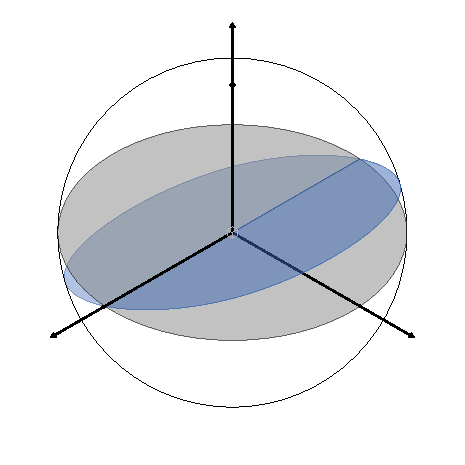
\includegraphics[width=0.4\linewidth]{graphics/test.pdf}
    \caption{Definition of a general Body-centered inertial (BCI) reference frame.}
    \label{fig:bci}
\end{figure}

\begin{figure}[h]
    \centering
    \def\svgwidth{0.4\linewidth}
    % \input{graphics/drawing2.pdf_tex}
    \import{graphics/}{test.pdf_tex}
    \caption{Definition of a general Body-centered inertial (BCI) reference frame.}
    \label{fig:my_label}
\end{figure}

%%%%%%%%%%%%%%%%%%%%%%%%%%%%%%%%%%%%%%%%%%%%%%%%%%%%%%%%%%%%%%%%%%%%%%%%%%%%%%%%
\subsection{Body-centered body-fixed (BCBF)\label{ssec:frame_bcbf}}
%%%%%%%%%%%%%%%%%%%%%%%%%%%%%%%%%%%%%%%%%%%%%%%%%%%%%%%%%%%%%%%%%%%%%%%%%%%%%%%%

The body-centered body-fixed (BCBF) reference frames are frames which have their
origins at the center of mass of a body, the $Z_F$-axis is directed along
(counter clockwise positive) spin-axis of the body. The $X_F$-axis passes
through the reference meridian of the body, which is at an angle of
$\Omega_t{t_0}$ from the ascending node of the intersection between the ecliptic
and the equator of the body. The $Y_F$-axis then passes through the equatorial
plane perpendicular to $X_F$ and $Z_F$.

\begin{figure}[!htp]
    \centering
    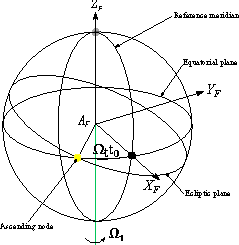
\includegraphics[width=0.35\linewidth]{graphics/bcbf.pdf}
    \caption{
        Definition of a general Body-centered body-fixed (BCBF) reference frame.
    }
    \label{fig:bci}
\end{figure}


\begin{equation}
    W = W_0 + \dot{W}d
    \label{eq:ephem_prime_meridian}
\end{equation}
\begin{equation*}
    \begin{aligned}
        \textrm{where, }
        W &= \textrm{the ephemeris position of the prime meridian} \\
        W_0 &= \textrm{the value of W at J2000.0 (occasionally some other epoch),} \\
        d &= \textrm{interval in days from the standard epoch.}
    \end{aligned}
\end{equation*}

\begin{equation}
    \mathbf{R}^{I/B}=\mathbf{R}_z(W)\mathbf{R}_x(\pi/2-\delta_0)\mathbf{R}_z(\pi/2-\alpha_0)
    \label{eq:bci_transformation}
\end{equation}
\begin{equation*}
    \begin{aligned}
        \textrm{where, }
        \mathbf{R}_{x,y,z}(\phi) &= \textrm{transformation matrix for a rotation of $\phi$ radians about the respective axis (\autoref{appendix:rotational_transformations}),}\\
        \alpha_0, \delta_0 &= \textrm{ICRF equatorial coordinates at epoch J2000.0} \\
    \end{aligned}
\end{equation*}

%%%%%%%%%%%%%%%%%%%%%%%%%%%%%%%%%%%%%%%%%%%%%%%%%%%%%%%%%%%%%%%%%%%%%%%%%%%%%%%%
\subsection{Radial tangential normal (RTN)\label{ssec:frame_rtn}\label{ssec:frame_rsw}}
%%%%%%%%%%%%%%%%%%%%%%%%%%%%%%%%%%%%%%%%%%%%%%%%%%%%%%%%%%%%%%%%%%%%%%%%%%%%%%%%

The radial tangential normal frame (RTN), a.k.a. the radial (R), along-track (S)
and cross-track (W) frame (RSW), is a dynamic frame with an orbiting spacecraft
at the centre of the frame. The frame is time dependent and based on the
two-body restricted problem problem with the R-component determined by the
current unit-vector of position $\hat{r}$, the T-component by the unit vector of
velocity $\hat{v}$, and the N-component by their the cross product of the two,
the specific angular momentum vector $\hat{r}\cross{\hat{v}}=\hat{h}$. This
frame is commonly used for relative motion of spacecraft in a rendezvous
segment.

\begin{equation}
    \mathbf{R}^{I/RSW}= \bigg[\hat{\mathbf{r}}_{B/S}\; \hat{\mathbf{v}}_{B/S}\; \hat{\mathbf{h}}_{B/S} \bigg]
\end{equation}
\begin{equation*}
    \begin{aligned}
        \textrm{where, }
        \hat{\mathbf{r}}_{B/S} &= \textrm{the position of the spacecraft with respect to the body,}\\
        \hat{\mathbf{v}}_{B/S} &= \textrm{the velocity of the spacecraft with respect to the body,}\\
        \hat{\mathbf{h}}_{B/S} &= \textrm{the specific angular momentum of the spacecraft with respect to the body,}\\
    \end{aligned}
\end{equation*}

%%%%%%%%%%%%%%%%%%%%%%%%%%%%%%%%%%%%%%%%%%%%%%%%%%%%%%%%%%%%%%%%%%%%%%%%%%%%%%%%
\section{Orbital Elements}
%%%%%%%%%%%%%%%%%%%%%%%%%%%%%%%%%%%%%%%%%%%%%%%%%%%%%%%%%%%%%%%%%%%%%%%%%%%%%%%%
Orbital elements are a set of parameters which uniquely define a Keplerian, or
two-body restricted orbit, around a given central body in the absence of any
external perturbations incurred in the system. This definition is given with
with respect to a plane of reference and a reference direction. Conversion
between any arbitrary pair of orbital elements of a given reference plane and
direction, requires only the central body's gravitational parameter $\mu$.

%%%%%%%%%%%%%%%%%%%%%%%%%%%%%%%%%%%%%%%%%%%%%%%%%%%%%%%%%%%%%%%%%%%%%%%%%%%%%%%%
\subsection{Cartesian}
%%%%%%%%%%%%%%%%%%%%%%%%%%%%%%%%%%%%%%%%%%%%%%%%%%%%%%%%%%%%%%%%%%%%%%%%%%%%%%%%
The Cartesian, a.k.a. the rectangular orbital elements are the concatenation of
the position and velocity vectors in the respectively named coordinate system
relative to the central body,

\begin{equation}
    \textrm{\OE}_C=
    \begin{bmatrix}
        \mathbf{r}^T &
        \mathbf{v}^T &
    \end{bmatrix}^T
    =
    \begin{bmatrix}
        r_x &
        r_y &
        r_z &
        v_x &
        v_y &
        v_z &
    \end{bmatrix}^T,
\end{equation}

where all values are assumed as S.I. units, where not specified otherwise, in
further calculations involving the orbital elements.

%%%%%%%%%%%%%%%%%%%%%%%%%%%%%%%%%%%%%%%%%%%%%%%%%%%%%%%%%%%%%%%%%%%%%%%%%%%%%%%%
\subsection{Keplerian}
%%%%%%%%%%%%%%%%%%%%%%%%%%%%%%%%%%%%%%%%%%%%%%%%%%%%%%%%%%%%%%%%%%%%%%%%%%%%%%%%
The Keplerian, a.k.a. the classical orbital elements are the

\begin{equation}
    \textrm{\OE}_K=
    \begin{bmatrix}
        a &
        e &
        i &
        \Omega &
        \omega &
        \theta &
    \end{bmatrix}^T,
\end{equation}

%%%%%%%%%%%%%%%%%%%%%%%%%%%%%%%%%%%%%%%%%%%%%%%%%%%%%%%%%%%%%%%%%%%%%%%%%%%%%%%%
\subsection{Modified Equinoctial}
%%%%%%%%%%%%%%%%%%%%%%%%%%%%%%%%%%%%%%%%%%%%%%%%%%%%%%%%%%%%%%%%%%%%%%%%%%%%%%%%
The Keplerian, a.k.a. the classical orbital elements are the

\begin{equation}
    \textrm{\OE}_{ME}=
    \begin{bmatrix}
        p &
        f &
        g &
        h &
        k &
        L
    \end{bmatrix}^T,
\end{equation}

\begin{equation}
    \begin{aligned}
        p=&a(1-e^2)\\
        f=&e\cos{(\omega+\Omega)}\\
        g=&e\cos{(\omega+\Omega)}\\
        h=&\tan{(i/2)}\cos{\Omega}\\
        k=&\tan{(i/2)}\sin{\Omega}\\
        L=&\Omega+\omega+\theta\\
    \end{aligned}
\end{equation}

\cite{Equinoctial}

%%%%%%%%%%%%%%%%%%%%%%%%%%%%%%%%%%%%%%%%%%%%%%%%%%%%%%%%%%%%%%%%%%%%%%%%%%%%%%%%
\section{Preliminary Orbit Determination}
%%%%%%%%%%%%%%%%%%%%%%%%%%%%%%%%%%%%%%%%%%%%%%%%%%%%%%%%%%%%%%%%%%%%%%%%%%%%%%%%

%%%%%%%%%%%%%%%%%%%%%%%%%%%%%%%%%%%%%%%%%%%%%%%%%%%%%%%%%%%%%%%%%%%%%%%%%%%%%%%%
\subsection{Gibbs method}
%%%%%%%%%%%%%%%%%%%%%%%%%%%%%%%%%%%%%%%%%%%%%%%%%%%%%%%%%%%%%%%%%%%%%%%%%%%%%%%%

%%%%%%%%%%%%%%%%%%%%%%%%%%%%%%%%%%%%%%%%%%%%%%%%%%%%%%%%%%%%%%%%%%%%%%%%%%%%%%%%
\subsection{Lambert's problem}
%%%%%%%%%%%%%%%%%%%%%%%%%%%%%%%%%%%%%%%%%%%%%%%%%%%%%%%%%%%%%%%%%%%%%%%%%%%%%%%%

%%%%%%%%%%%%%%%%%%%%%%%%%%%%%%%%%%%%%%%%%%%%%%%%%%%%%%%%%%%%%%%%%%%%%%%%%%%%%%%%
\subsection{Gauss method}
%%%%%%%%%%%%%%%%%%%%%%%%%%%%%%%%%%%%%%%%%%%%%%%%%%%%%%%%%%%%%%%%%%%%%%%%%%%%%%%%

%%%%%%%%%%%%%%%%%%%%%%%%%%%%%%%%%%%%%%%%%%%%%%%%%%%%%%%%%%%%%%%%%%%%%%%%%%%%%%%%
\section{Orbital Perturbations}
%%%%%%%%%%%%%%%%%%%%%%%%%%%%%%%%%%%%%%%%%%%%%%%%%%%%%%%%%%%%%%%%%%%%%%%%%%%%%%%%
In order to account for perturbations such as a non-spherical body, atmospheric
drag, propulsive thrust, solar radiation pressure, and other celestial objects
outside the two-body formulation, \autoref{eq:newtons_equation_planetary} can be
rewritten as

\begin{equation}
    \ddot{\mathbf{r}}=\frac{\mu}{|\mathbf{r}|^3}\mathbf{r}+\mathbf{p},
    \label{eq:newtons_equation_planetary_with_p}
\end{equation}
where $\mathbf{p}$ is the net perturbative accelerations from all sources other than the spherically symmetric gravitational attraction between the two bodies.

%%%%%%%%%%%%%%%%%%%%%%%%%%%%%%%%%%%%%%%%%%%%%%%%%%%%%%%%%%%%%%%%%%%%%%%%%%%%%%%%
\subsection{Cowell's method}
%%%%%%%%%%%%%%%%%%%%%%%%%%%%%%%%%%%%%%%%%%%%%%%%%%%%%%%%%%%%%%%%%%%%%%%%%%%%%%%%

\begin{equation}
    \begin{aligned}
        \ddot{\mathbf{r}}=\dv{\dot{\mathbf{r}}}{t}=-\frac{\mu}{r^3}\mathbf{r} + \mathbf{p}
    \end{aligned}
\end{equation}

%%%%%%%%%%%%%%%%%%%%%%%%%%%%%%%%%%%%%%%%%%%%%%%%%%%%%%%%%%%%%%%%%%%%%%%%%%%%%%%%
\subsection{Encke's method}
%%%%%%%%%%%%%%%%%%%%%%%%%%%%%%%%%%%%%%%%%%%%%%%%%%%%%%%%%%%%%%%%%%%%%%%%%%%%%%%%

%%%%%%%%%%%%%%%%%%%%%%%%%%%%%%%%%%%%%%%%%%%%%%%%%%%%%%%%%%%%%%%%%%%%%%%%%%%%%%%%
\subsection{Variational Equations: Lagrange Planetary}
%%%%%%%%%%%%%%%%%%%%%%%%%%%%%%%%%%%%%%%%%%%%%%%%%%%%%%%%%%%%%%%%%%%%%%%%%%%%%%%%

\begin{equation}
    \begin{aligned}
        \dv{a}{t}&=-\frac{2a^2}{\mu}\pdv{R}{t_p}\\
        \dv{e}{t}&=-\frac{\sqrt{1-e^2}}{\sqrt{\mu{a}}e}\pdv{R}{a} + \frac{a(1-e^2)}{\mu{e}} \pdv{R}{t_p}\\
        \dv{t_p}{t}&=\frac{2a^2}{\mu}\pdv{R}{a}+\frac{a(1-e^2)}{\mu{e}}\pdv{R}{e}\\
        \dv{\Omega}{t}&=\frac{1}{\sqrt{\mu{a}(1-e^2)}\sin{i}}\pdv{R}{i}\\
        \dv{i}{t}&=\frac{1}{\sqrt{\mu{a(1-e^2)}}}\bigg(\frac{1}{\tan{i}}\pdv{R}{\omega}-\frac{1}{\sin{i}}\pdv{R}{\Omega}\bigg)\\
        \dv{\omega}{t}&=-\frac{1}{\sqrt{\mu{a}(1-e^2)\tan{i}}}\pdv{R}{i}+\frac{\sqrt{1-e^2}}{\sqrt{\mu{a}}e}\pdv{R}{e}
    \end{aligned}
\end{equation}

%%%%%%%%%%%%%%%%%%%%%%%%%%%%%%%%%%%%%%%%%%%%%%%%%%%%%%%%%%%%%%%%%%%%%%%%%%%%%%%%
\subsection{Variational Equations: Gauss}
%%%%%%%%%%%%%%%%%%%%%%%%%%%%%%%%%%%%%%%%%%%%%%%%%%%%%%%%%%%%%%%%%%%%%%%%%%%%%%%%

\begin{equation}
    \begin{aligned}
        \dv{a}{t}&=2\sqrt{\frac{a}{\mu}}\bigg(F_R\frac{ae}{\sqrt{1-e^2}}\sin{\theta}+F_S\frac{a^2\sqrt{1-e^2}}{a(1-e\cos{E})}\bigg)\\
        \dv{e}{t}&=\frac{h}{\mu}\sin{\theta}F_R+\frac{1}{\mu{h}}\bigg((h^2+\mu{r})\cos{\theta}+\mu{r}\bigg)F_S\\
        \dv{i}{t}&=\frac{r}{h}\cos{(\omega+\theta)}F_W\\
        \dv{\Omega}{t}&=\frac{r}{h\sin{i}}\sin{(\omega+\theta)}F_W\\
        \dv{\omega}{t}&=-\frac{1}{eh}\bigg(\frac{h^2}{\mu}\cos{\theta}F_R-(r+\frac{h^2}{\mu}\sin{\theta}F_S)\bigg)-\frac{r\sin{\omega+\theta}}{h\tan{i}}F_W\\
        \dv{\theta}{t}&=\frac{h}{r^2}+\frac{1}{eh}\bigg(\frac{h^2}{\mu}\cos{\theta}F_R-(r+\frac{h^2}{\mu})\sin{\theta}F_S\bigg)
    \end{aligned}
\end{equation}

\begin{equation}
    \begin{aligned}
        \dv{p}{t}&=\frac{2p}{w}\sqrt{\frac{p}{\mu}}F_R\\
        \dv{f}{t}&=\sqrt{\frac{p}{\mu}}\bigg(F_R\sin{L}+[(w+1)\cos{L}+f]\frac{F_T}{w}-(h\sin{L}-k\cos{L})\frac{gF_N}{w}\bigg)\\
        \dv{g}{t}&=\sqrt{\frac{p}{\mu}}\bigg(-F_R\cos{L}+[(w+1)\sin{L}+g]\frac{F_T}{w}-(h\sin{L}-k\cos{L})\frac{gF_N}{w}\bigg)\\
        \dv{h}{t}&=\sqrt{\frac{p}{\mu}}\frac{s^2F_N}{2w}\sin{L}\\
        \dv{k}{t}&=\sqrt{\frac{p}{\mu}}\frac{s^2F_N}{2w}\cos{K}\\
        \dv{L}{t}&=\sqrt{\mu{p}}\bigg(\frac{w}{p}\bigg)^2+\frac{1}{w}\sqrt{\frac{p}{\mu}}(h\sin{L}-k\cos{L})F_N\\
    \end{aligned}
\end{equation}


% \subsubsection{Analytical Methods}


% \subsubsection{Tracking Methods}
% The orbit determination of an artificial satellite requires empirical observations related to the satellites position of velocity. These observations are collected by a satellites tracking system with the use of electromagnetic wave propagation between a transmitter and a receiver. Each observation corresponding to a unique pair of transmitter and receiver can be generalised as a \textbf{link}.

% % \subsubsection{Radar Tracking}

% % https://solarsystem.nasa.gov/basics/chapter18-1/
% \subsubsection{Deep Space Network (DSN)}

% \cite{Berner2007}

% \begin{itemize}
%     \item \textbf{Frequency \& Timing Data Type, F\&T}
%     \item \textbf{Tracking Data Type, TRK}
%     \item \textbf{Telemetry Data Type, TLM}
%     \item \textbf{Command Data Type, CMD}
%     \item \textbf{Monitor Data Type, MON}
%     \item \textbf{Radio Science Data Type, RS}
%     \item \textbf{Very Long Baseline Interferometry Data Type, VLBI}
% \end{itemize}

% \subsubsection{ESA's tracking station network (Estrack)}


